\documentclass[a4paper]{article}

%% Language and font encodings
\usepackage[english]{babel}
\usepackage[utf8x]{inputenc}
\usepackage[T1]{fontenc}

%% Sets page size and margins
\usepackage[a4paper,top=3cm,bottom=2cm,left=3cm,right=3cm,marginparwidth=1.75cm]{geometry}

%% Useful packages
\usepackage{ladder}
\usepackage{hyperref}
\usepackage{xcolor}
\usepackage{minted}

\definecolor{LG}{HTML}{F9F9F9}

%% Informations
\title{\textsf{ladder} package}
\author{Aurélien CADIOU \\ \href{mailto:contact@aureliencadiou.fr}{contact@aureliencadiou.fr}}

\begin{document}
\maketitle

\setcounter{tocdepth}{1}
\tableofcontents

\section*{Introduction}
This package permit the creation of simple ladder diagram into TeX documents.

\href{https://github.com/AurelienC/tex-ladder}{Github repository : tex-ladder}

\section{Installation}
Install this package like any other \LaTeX~package.

\section{Dependencies}
This package depends on :
\begin{itemize}
\item \href{https://www.ctan.org/search/?phrase=tikz}{tikz}
\item \href{https://www.ctan.org/pkg/ifthen}{ifthen}
\item \href{https://www.ctan.org/pkg/calc}{calc}
\end{itemize}


\section{Usage}
\subsection{Package}
Add following packages on your document : \mintinline{latex}{\usepackage{tikz} \usepackage{ladder}}.


\subsection{Net}
All contacts and relays are, by default, added in serie.
\begin{itemize}
\item \mintinline{latex}{\ladderLine} begin a new ladder net
\item \mintinline{latex}{\startParallel} begin a parallel segment
\item \mintinline{latex}{\setParallel} begin the new parallel segment
\item \mintinline{latex}{\unsetParallel} end of the parallel segment
\end{itemize}

\subsection{Contacts}
\texttt{type} of contacts may be any letter. Conventionnaly, we use \texttt{P} for rising edge contact and \texttt{N} for falling edge contact.\\

\begin{itemize}
\item \mintinline{latex}{\ladderNO[type]{name}{mnemonic}}  Normally Opened contact
\item \mintinline{latex}{\ladderNC[type]{name}{mnemonic}}  Normaly Closed contact 
\end{itemize}
   

\subsection{Coils}
\texttt{type} of coils may be any letter. Conventionnaly, we use \texttt{R} for reset coil, \texttt{S} for set coil.\\

\begin{itemize}
\item \mintinline{latex}{\ladderC[type]{name}{mnemonic}} a coil 
\end{itemize}


\section{Simple example}
\subsection{Preview}
\begin{figure}[h!]
    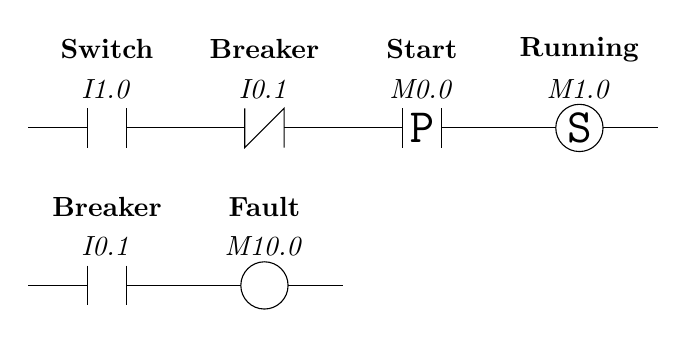
\begin{tikzpicture}
      \ladderLine
      \ladderNO{Switch}{I1.0}
      \ladderNC{Breaker}{I0.1}
      \ladderNO[P]{Start}{M0.0}
      \ladderC[S]{Running}{M1.0}
      
      \ladderLine
      \ladderNO{Breaker}{I0.1}
      \ladderC{Fault}{M10.0}
    \end{tikzpicture}
	\caption{Example with contacts and coil}
    \label{example1}
\end{figure}

\subsection{Code}
Code of figure \ref{example1}.
\begin{minted}[bgcolor=LG, fontsize=\footnotesize]{latex}
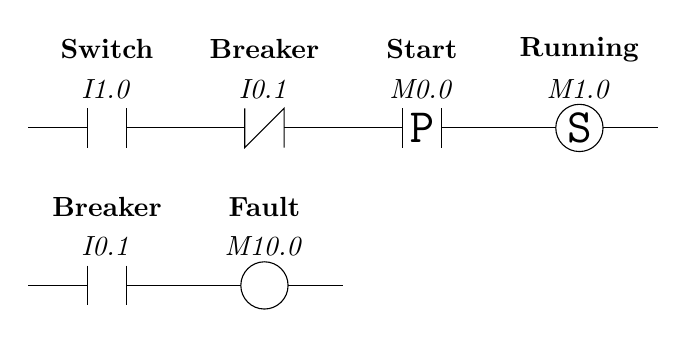
\begin{tikzpicture}
  \ladderLine
    \ladderNO{Switch}{I1.0}
    \ladderNC{Breaker}{I0.1}
    \ladderNO[P]{Start}{M0.0}
    \ladderC[S]{Running}{M1.0}

  \ladderLine
    \ladderNO{Breaker}{I0.1}
    \ladderC{Fault}{M10.0}
\end{tikzpicture}
\end{minted}


\section{Parallel section}
\subsection{Preview}
\begin{figure}[h!]
    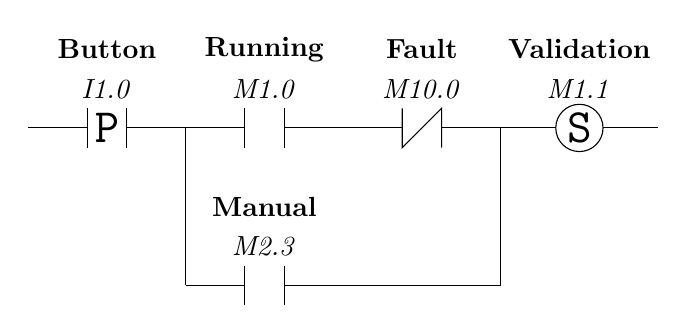
\begin{tikzpicture}
      \ladderLine
        \ladderNO[P]{Button}{I1.0}

        \startParallel % Begin of section
          \ladderNO{Running}{M1.0} 
          \ladderNC{Fault}{M10.0}

        \setParallel
        	\ladderNO{Manual}{M2.3}
        \unsetParallel

        \ladderC[S]{Validation}{M1.1}
    \end{tikzpicture}
	\caption{Example with parallel section}
    \label{example2}
\end{figure}

\subsection{Code}
Code of figure \ref{example2}.

\begin{minted}[bgcolor=LG, fontsize=\footnotesize]{latex}
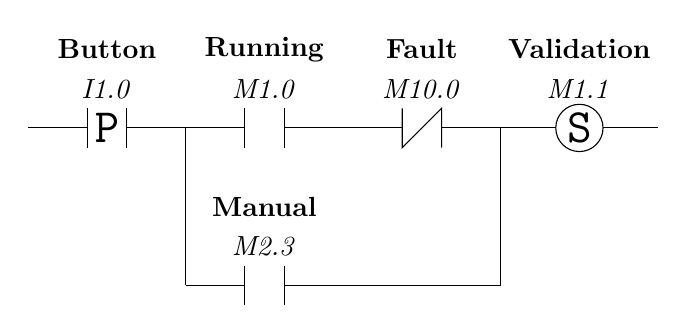
\begin{tikzpicture}
	\ladderLine
		\ladderNO[P]{Button}{I1.0}

		\startParallel % Begin of section
			\ladderNO{Running}{M1.0} 
			\ladderNC{Fault}{M10.0}

		\setParallel
			\ladderNO{Manual}{M2.3}
		\unsetParallel

		\ladderC[S]{Validation}{M1.1}
\end{tikzpicture}
\end{minted}




\section{Complete example}
\subsection{Preview}
\begin{figure}[!h]
    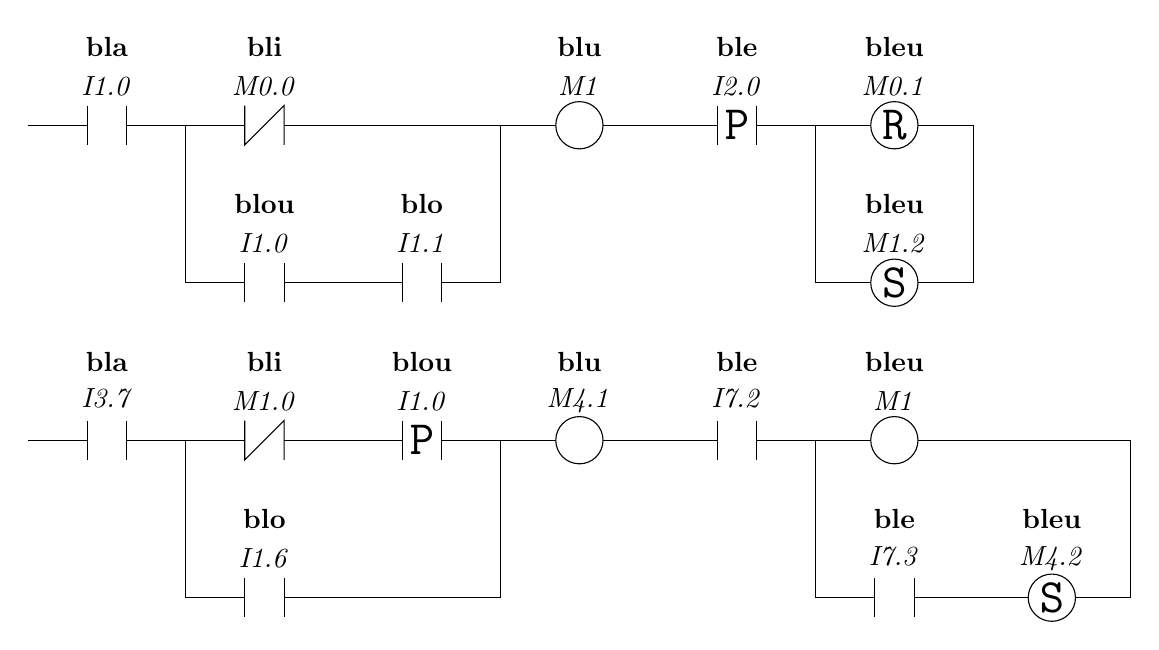
\begin{tikzpicture}
    \ladderLine % Begenning new line
    \ladderNO{bla}{I1.0}

    % M0 will be in parallel with I1.0 and I1.1
    \startParallel 
    \ladderNC{bli}{M0.0}

    \setParallel 
      \ladderNO{blou}{I1.0}
      \ladderNO{blo}{I1.1}
    \unsetParallel

    \ladderC{blu}{M1} % On met une "bobine"
    \ladderNO[P]{ble}{I2.0}

    \startParallel
    \ladderC[R]{bleu}{M0.1}
    \setParallel
    
      \ladderC[S]{bleu}{M1.2}
    \unsetParallel

    % New section
    \ladderLine

    \ladderNO{bla}{I3.7}

    \startParallel
    \ladderNC{bli}{M1.0}
    \ladderNO[P]{blou}{I1.0}

    \setParallel
        \ladderNO{blo}{I1.6}
    \unsetParallel

    \ladderC{blu}{M4.1}

    \ladderNO{ble}{I7.2}

    \startParallel
    \ladderC{bleu}{M1}{R}

    \setParallel
      \ladderNO{ble}{I7.3}
      \ladderC[S]{bleu}{M4.2}
    \unsetParallel
  \end{tikzpicture}
  \caption{Example of ladder package usage}
  \label{example3}
\end{figure}

\subsection{Code}
Code of figure \ref{example3}.

\begin{minted}[bgcolor=LG, fontsize=\footnotesize]{latex}
\begin{figure}
    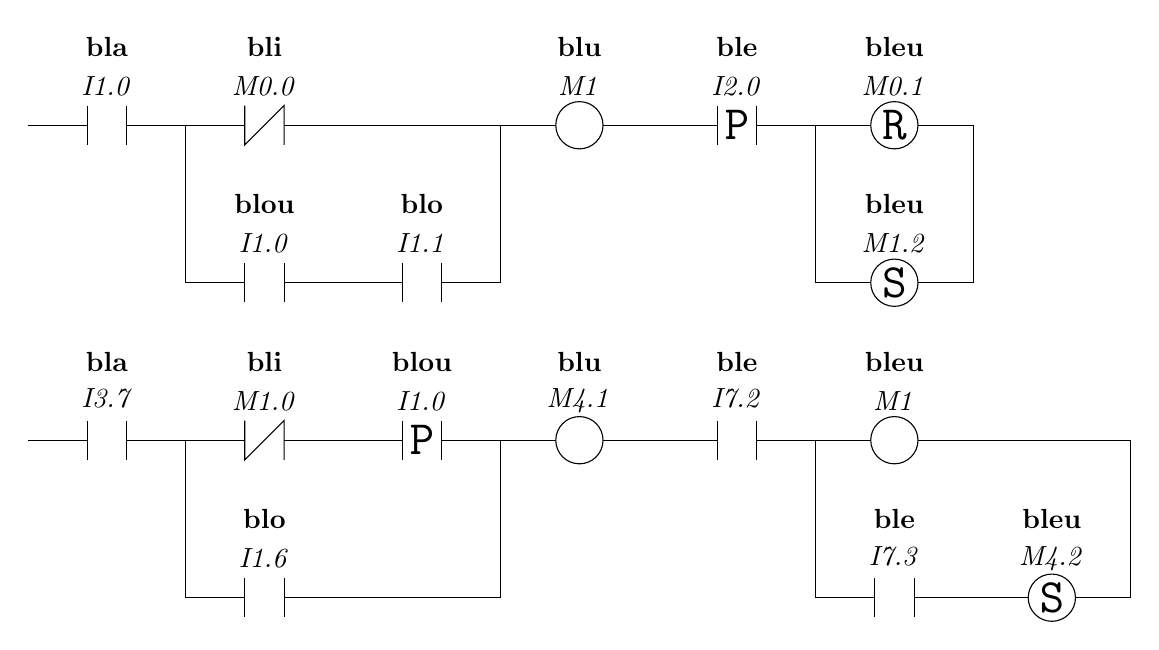
\begin{tikzpicture}
    \ladderLine % Begenning new line
    \ladderNO{bla}{I1.0}

    % M0 will be in parallel with I1.0 and I1.1
    \startParallel 
    \ladderNC{bli}{M0.0}

    \setParallel 
      \ladderNO{blou}{I1.0}
      \ladderNO{blo}{I1.1}
    \unsetParallel

    \ladderC{blu}{M1} % On met une "bobine"
    \ladderNO[P]{ble}{I2.0}

    \startParallel
    \ladderC[R]{bleu}{M0.1}
    \setParallel
      \ladderC[S]{bleu}{M1.2}
    \unsetParallel

    % New section
    \ladderLine

    \ladderNO{bla}{I3.7}

    \startParallel
    \ladderNC{bli}{M1.0}
    \ladderNO[P]{blou}{I1.0}

    \setParallel
        \ladderNO{blo}{I1.6}
    \unsetParallel

    \ladderC{blu}{M4.1}

    \ladderNO{ble}{I7.2}

    \startParallel
    \ladderC{bleu}{M1}{R}

    \setParallel
      \ladderNO{ble}{I7.3}
      \ladderC[S]{bleu}{M4.2}
    \unsetParallel
  \end{tikzpicture}
  \caption{Example of ladder package usage}
\end{figure}
\end{minted}


\end{document}